\documentclass[xcolor=pdftex,dvipsnames,table,10pt,babel,spanish]{beamer}

\usetheme{Warsaw}

\usepackage[spanish]{babel}
\usepackage[latin1]{inputenc}
\usepackage{stmaryrd}
\usepackage{graphicx}

\usepackage{listings}


\usepackage{setspace}

\usepackage{color}
\usepackage{textcomp}
\definecolor{listinggray}{gray}{0.9}
\definecolor{lbcolor}{rgb}{0.95,0.95,0.95}
\lstset{
    backgroundcolor=\color{lbcolor},
    tabsize=4,6
    rulecolor=,
    language=matlab,
        basicstyle=\scriptsize,
        upquote=true,
        aboveskip={1.5\baselineskip},
        columns=fixed,
        showstringspaces=false,
        extendedchars=true,
        breaklines=true,
        prebreak = \raisebox{0ex}[0ex][0ex]{\ensuremath{\hookleftarrow}},
        frame=single,
        showtabs=false,
        showspaces=false,
        showstringspaces=false,
        identifierstyle=\ttfamily,
        keywordstyle=\color[rgb]{0.1,0.1,0.6}\bfseries,
        commentstyle=\color[rgb]{0.133,0.545,0.133},
        stringstyle=\color[rgb]{0.627,0.126,0.941},
}


\setbeamercovered{transparent}

\title{A Framework for Small Distributed Projects}
\subtitle{And a Protein Clusterer Application}
\author{Guillermo Biset}
\pgfdeclareimage[height=2.5cm]{unrc}{images/escudo.jpg}
\pgfdeclareimage[height=2.5cm]{fud}{images/fud_logo.png}
\pgfdeclareimage[height=2.5cm]{fudepan}{images/logo-fudepan.png}

\institute[U.N.R.C.]{
  \textsc{Departamento de Computaci\'on} \\
  \textsc{Universidad Nacional de R\'io Cuarto} \\
  \ \\
  \pgfuseimage{unrc}  \qquad \qquad \pgfuseimage{fud} \qquad \qquad \pgfuseimage{fudepan}}

\date{}

\begin{document}

\frame{\titlepage}

\frame{
\frametitle{Temario: }
\tableofcontents
}

\section{Motivaci\'on y Problema}

\subsection{FuD}

        \frame{
            \frametitle{Motivaci\'on}
            \begin{block}{}
            El uso de recursos computacionales es transversal a la mayor\'ia de las ciencias aplicadas.
            \end{block}

            \pause
            
            \begin{block}{}
            Muchos de estos usos presentan requerimientos de procesamiento de un conjunto considerable de datos.
            \end{block}

            \pause
            
            \begin{block}{}
            Un buen enfoque a la hora de procesar eficientemente un gran conjunto de datos es mediante t\'ecnicas computacionales de paralelizaci\'on.
            \end{block}
            
            \pause
            
            \begin{block}{}
            El \textbf{problema}, sin embargo, es que los cient\'ificos especialistas en los problemas a resolver no necesariamente son especialistas en programaci\'on paralela.
            \end{block}

        }

        \frame{
          \frametitle{Problema}
          
          Se desea, entonces, desarrollar un marco de aplicaci\'on (o framework) que permita, a cient\'ificos no especialistas en t\'ecnicas de paralelizaci\'on, implementar soluciones inform\'aticas para sus problemas  con las siguientes caracter\'isticas:
          \begin{itemize}
          \pause
          \item No debe ser necesario poseer conocimientos avanzados de programaci\'on ni concurrencia.
          \pause
          \item Se deben aprovechar los beneficios de la programaci\'on paralela mediante el uso del framework.
          \pause
          \item El uso del framework no debe imponer serias desventajas de performance.
          \pause
          \item El framework debe aprovechar diferentes disposiciones de los recursos computacionales.
          \end{itemize}
        }

    \begin{frame}
     \frametitle{Enfoques Similares}
     
     Existen varios enfoques que permiten, parcialmente, tratar estos problemas:
     
     \begin{block}{Enfoques notables}
     \begin{description}
     \item [BOINC]: Es un middleware no comercial dise\~nado en Berkeley para computaci\'on voluntaria y grid\cite{boinc1}
     \pause
     \item [MPI]: Es una interfaz que permite que muchas computadoras se comuniquen entre s\'i principalmente utilizada en clusters de alta performance\cite{mpi}
     \pause
     \item [MapReduce]: Es un modelo de programaci\'on desarrollado en Google para permitir la implementaci\'on de algoritmos distribu\'idos\cite{mapreduce}.
     \end{description}

     \end{block}

    \end{frame}


\subsection{El clusterer}

        \frame{
          \frametitle{El clusterer de prote\'inas}
          
          \begin{block}{}
          En \textbf{FuDePAN}, un proyecto (Galadriel) se encarga de generar estructuras de prote\'inas autom\'aticamente, sujetas a viabilidad tridimensional.
          \end{block}

          \pause
          
          Pero la mayor\'ia de estas estructuras generadas presentan similitudes geom\'etricas al punto de evidenciar comportamiento id\'entico ante aplicaciones medicinales.
          
          \pause
          
          \begin{block}{}
          Se debe, entonces, tomar datos generados por Galadriel y realizar agrupaciones de estas estructuras basados en sus similitudes geom\'etricas, para permitir a los investigadores concentrarse solamente en alguna de estas prote\'inas.
          \end{block}

          }
          

\section{Marco Te\'orico}

\subsection{Programaci\'on en Paralelo}

  \frame{
    \frametitle{Programaci\'on en Paralelo}
    
    La programaci\'on en paralelo se refiere a algoritmos y programas que se ejecutan en computadoras paralelas, aunque hay varias presentaciones diferentes que constituyen a una computadora paralela, una definici\'on aceptada es la siguiente\cite{parallel}:
    
    \pause

    \begin{block}{}
    Una computadora paralela es un conjunto de procesadores que pueden trabajar de manera cooperativa para resolver un problema computacional.
    \end{block}
    
    \pause 
    
    \begin{block}{}
    Esta definici\'on es lo suficientemente amplia para incluir supercomputadoras con cientos o miles de procesadores, redes amplias de computadoras o clusters centralizados de ellas.
    \end{block}

  }

  \frame{
    \frametitle{La taxonom\'ia de Flynn}
    
    Flynn\cite{flynn} propuso una taxonom\'ia de arquitecturas de computadoras basado en la cantidad de instrucciones que se pueden ejecutar concurrentemente y la cantidad de flujos de datos disponibles distinguiendo los siguientes casos:
    
    \begin{description}
    \item [Single Instruction, Single Data stream] (o SISD): Una computadora seceuncial que no explota el paralelismo en cuantos a instrucciones o datos.

    \pause

    \item [Single Instruction, Multiple Data streams] (o SIMD): Una computadora que utiliza manejo paralelo de datos sobre un \'unico nodo de procesamiento.

    \pause

    \item [Multiple Instruction, Single Data stream] (o MISD): Referido a m\'ultiples nodos de procesamiento que utilizan un \'unico repositorio de datos.

    \pause

    \item [Multiple Instruction, Multiple Data streams] (o MIMD): Cuando m\'ultiples procesadores hacen uso de datos ubicados en de manera distribu\'ida.
    \end{description}

  }

    \frame{
      \frametitle{SISD}
      
      \begin{center}
      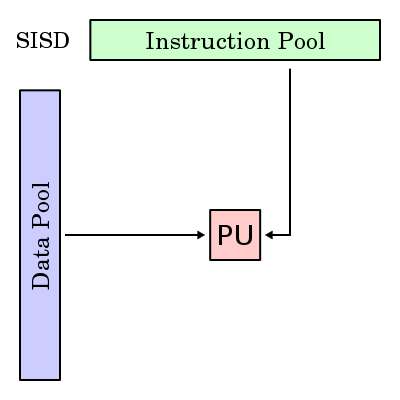
\includegraphics[height=5cm]{images/SISD.png}
      \end{center}

    }

    \frame{
      \frametitle{SIMD}
      
      \begin{center}
      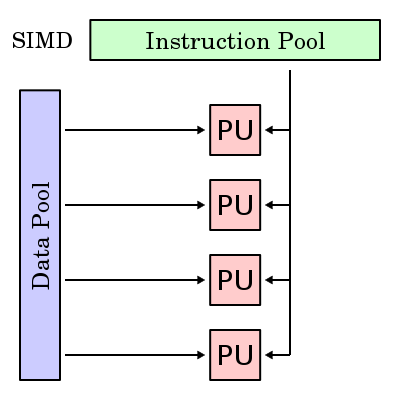
\includegraphics[height=5cm]{images/SIMD.png}
      \end{center}

    }
    
    \frame{
      \frametitle{MISD}
      
      \begin{center}
      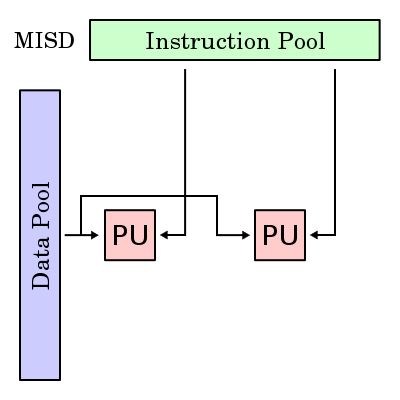
\includegraphics[height=5cm]{images/MISD.png}
      \end{center}

    }
    
    \frame{
      \frametitle{MIMD}
      
      \begin{center}
      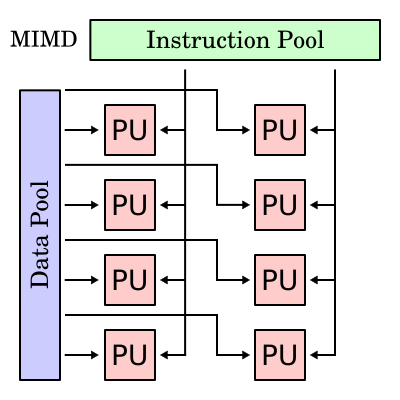
\includegraphics[height=5cm]{images/MIMD.png}
      \end{center}

    }


\subsection{Clustering}

  \frame{
    \frametitle{Clustering}
    
    El clustering de datos se realiza con el prop\'osito de agrupar objetos bajo ciertas propiedades que estos evidencian. Una definici\'on aceptada, tomada de \cite{clustering} es la siguiente:
    
    \pause
    
    \begin{block}{Data Clustering}
    El clustering de datos (o clustering) es un m\'etodo para crear grupos de objetos (o clusters) de tal modo que los objetos en un cluster son muy similares entre s\'i y objetos en grupos diferentes son bastante diferentes.
    \end{block}

    \pause
    
    De manera m\'as formal:
    
    \begin{block}{}
    El clustering de datos se realiza sobre un determinado conjunto de datos utilizando una noci\'on de similitud dada mediante la agrupaci\'on de los datos de manera que los elementos en un mismo grupo son similares para esta noci\'on y elementos de diferentes grupos son diferentes.
    \end{block}

  }

\begin{frame}[fragile]
 \frametitle{Algoritmo \emph{k}-means}

\lstset{language=Pascal}
\begin{lstlisting}[frame=single]
Require: Data set D, Number of clusters k, Dimensions d:
  {Ci is the ith cluster}
  {1. Initialization Phase}
1 : (C1,C2,...,Ck) := Initial partition of D.
  {2. Iteration Phase}
2 : repeat
3 :     dij := distance between case i and cluster j;
4 :     ni  := arg min 1<=j<=k dij;
5 :     Assign case i to cluster ni;
6 :     Recompute the cluster means of any changed clusters above;
7 : until no further changes of cluster membership occur
8 : Output Results
\end{lstlisting}
\centering {The conventional \emph{k}-means algorithm.} 
\label{k-means}


\end{frame}

\subsection*{Prote\'inas}

  \frame{
    \frametitle{Prote\'inas}
    
    Las prote\'inas son pol\'imeros de amino\'acidos unidos entre s\'i de forma lineal mediante uniones p\'eptidicas. 
    
    Una prote\'ina posee tres tipos de estructuras b\'asicas:
    
    \pause
    
    \begin{description}
    \item[Primaria]: La secuencia de amino\'acidos.
    \pause
    \item[Secundaria]: Se refiere al plegamiento de estructuras locales que se repiten regularmente, estabilizadas por uniones del tipo hidr\'ogeno.
    \pause
    \item[Terciaria]: Refiere a la forma general de una mol\'ecula individual y las relaciones espaciales que las estructuras secundarias tienen entre s\'i.
    \end{description}
    
  }

\subsection*{C++}

\begin{frame}[fragile]
  \frametitle{C++}
    
C++ es un lenguaje de programaci\'on de tipado est\'atico, multi paradigma, de prop\'osito general y compilado. Se lo reconoce como un lenguaje de nivel-medio, ya que es provee una combinaci\'on de capacidades de lenguajes de bajo y alto nivel.

\lstset{language=C++}
\begin{lstlisting}[frame=single]
//exception if _ids_to_job_map[id] isn't defined
mili::find(_ids_to_job_map,id)->process_results(id, message);

//remove from pending list
std::list<JobUnit*>::iterator it;
it = find_if(_pendingList.begin(),_pendingList.end(), 
             boost::bind(&JobUnit::get_id, _1) == id);

if (it != _pendingList.end())
{
    delete *it;
    _pendingList.erase(it);
}
else
    syslog(LOG_NOTICE,"Finished JobUnit % u was not pending.",id);
\end{lstlisting}


\end{frame}

\section{FuD}

    \frame{
      \frametitle{Raz\'on del framework}
      
      El framework (\textbf{FuD}) se desarroll\'o para contemplar el problema expresado previamente: permitir a cient\'ificos no especialistas en ciencias de la computaci\'on implementar de manera sencilla soluciones inform\'aticas que hagan uso de t\'ecnicas distribu\'idas de programaci\'on.
      
      Esto se puede resumir en el siguiente objetivo:
      
      \pause
      
      \begin{block}{}
      Dise\~ne y desarrolle un framework para automatizar la distribuci\'on de aplicaciones computacionales a trav\'es de disposiciones heterog\'eneas y din\'amicas de nodos de procesamiento.
      \end{block}
      
      \pause
      
      Adem\'as, el dise\~no deber\'ia:
      \begin{itemize}
       \item Ser lo suficientemente flexible para permitir desarrollar cualquier tipo de problema computacional.
       \pause
       \item Esta implementaci\'on debe ser independiente de los recursos que se dispondr\'an eventualmente par llevar a cabo el c\'omputo.
      \end{itemize}

    }

    \frame{
      \frametitle{Resumiendo}
      
      En resumen, \textbf{FuD} debe permitir ser utilizado para resolver cualquier problema que se puede solucionar secuencialmente. Adem\'as, debe permitir esto sin requerir que el implementador:
      
      \begin{itemize}
      \item Sepa conceptos de programaci\'on paralela.
      \pause
      \item Quede restringido a una determinada disposici\'on de los nodos procesadores.
      \pause
      \item Quede limitado por un particular sistema de comunicaci\'on.
      \end{itemize}

      \pause

      Finalmente, \textbf{FuD} asegura:
      \begin{itemize}
      \item Que la aplicaci\'on implementada tiene el potencial de ejecutarse paralelamente.
      \pause
      \item Que la aplicaci\'on explotar\'a los recursos que se pongan a su disposici\'on.
      \pause
      \item El uso del framework no generar\'a p\'erdidas de performance considerables.
      \pause
      \item Los datos intercambiados entre aplicaciones cliente y servidor no llevar\'an una carga adicional significativa sobre los datos necesarios para la aplicaci\'on.
      \end{itemize}

    }

  \frame{
    \frametitle{Enfoque}
    
    Para lograr esto, se debe implementar un esquema \emph{Divide\&Conquer}, donde el procesamiento ser\'a llevado a cabo por los nodos procesadores (o clientes):
    
    \pause 
    
    \begin{block}{\emph{Divide\&Conquer + Process}}
    \begin{description}
     \item [Divide]: Cuando se realiza la divisi\'on de un trabajo en una unidad de trabajo. Esto debe ser un proceso \emph{transaccional} y est\'a implementado por el m\'etodo \texttt{produce\_next\_job\_unit(size)}.
     \pause
     \item [Conquer]: Se lleva a cabo al incorporar los resultados de una unidad de trabajo, mediante \texttt{handle\_results(id, input)}.
     \pause
     \item [Process]: Las unidades de trabajo son comunicadas a un cliente, este las procesa y comunica los resultados para ser incorporados.
    \end{description}

    \end{block}

  }

\subsection{Dise\~no}

  \frame{
    \frametitle{Principios Utilizados}
    
    \begin{description}
    \item[SRP]: (o Single Responsibility Principle) No deber\'ia haber m\'as de una raz\'on de cambio para una clase.
    \pause
    \item[DIP]: (o Dependency Inversion Principle) Argumenta:
    \begin{itemize}
    \item M\'odulos de alto nivel no deber\'ian depender de m\'odulos inferiores, ambos deber\'ian depender de abstracciones.
    \item Las abstracciones no deber\'ian depnder de detalles, sino que los detalles deber\'ian depender de las abstracciones.
    \end{itemize}
    \pause
    \item[ISP]: (o Interface Segregation Principle) Los clientes no deber\'ian depender de interfases que no utilizar\'an.
    \pause
    \item[LSV]: (o Liskov Substitution Principle) Funciones que usan punteros o referencias a clases base deben poder utilizar objetos de subclases de la original sin saberlo.
    \end{description}

  }

  \frame{
    \frametitle{Conceptos centrales a \textbf{FuD} }
    
    \textbf{FuD} se organiza con un esquema Master-Worker (un servidor y varios clientes conectados al mismo). Los siguientes conceptos sirven para entender el funcionamiento de una aplicaci\'on que usa el framework:
    
    \begin{description}
    \item[Cliente]: Un cliente es una aplicaci\'on conectada al servidor y es el encargado de realizar las tareas de procesamiento.
    \pause
    \item[Trabajo]: Un trabajo es cualquier tarea a realizar por la aplicaci\'on (tambi\'en llamado trabajo distribu\'ible). Los mismos se pueden subdividir en unidades de trabajo.
    \pause
    \item[Unidad de Trabajo]: Representa un c\'omputo concreto y pertenece a un trabajo particular. No se puede dividir.
    \pause
    \item[El manejador de clientes]: Este m\'odulo es el encargado de manejar los clientes conectados al servidor.
    \pause
    \item[Manejador de trabajos]: Este es el m\'odulo de \textbf{FuD} encargado de llevar cuenta de los trabajos (de ambos tipos) que maneja el framework en un momento dado.
    \end{description}

  }

  \frame{
    \frametitle{Capas del framework }
    
    \textbf{FuD} se divide en 3 capas bien separadas. La siguiente figura ilustra esta caracter\'istica:
    
    \begin{center}
    \includegraphics [height=5cm]{images/abslayers.jpg}
    \end{center}
  }
  
  \frame{
    \frametitle{Capas del framework}
    
    \begin{description}
    \item[Aplicaci\'on]: Esta capa provee componentes que contienen todos los aspectos del dominio del problema. Como tal, incluye las definiciones y manejo de los datos usados y el algoritmo relevante a la soluci\'on implementada.
    \pause
    \item[Manejo de trabajo]: Esta capa se encarga de manejar ambos tipos de trabajo, haciendo de nexo entre la aplicaci\'on, donde se encuentran los trabajos concretos y se producen las unidades de trabajo, y los clientes, que se manejan en la capa inferior.
    \pause
    \item[Comunicaci\'on]: En esta capa existe el \'unico v\'inculo real entre clientes y servidor, la responsabilidad de esta capa es manejar los clientes conectados al servidor y llevar acabo los procedimientos de comunicaci\'on entre ambas aplicaciones.        
    \end{description}

  }

  \frame{
    \frametitle{Diagrama de clases}
    
    \begin{center}
    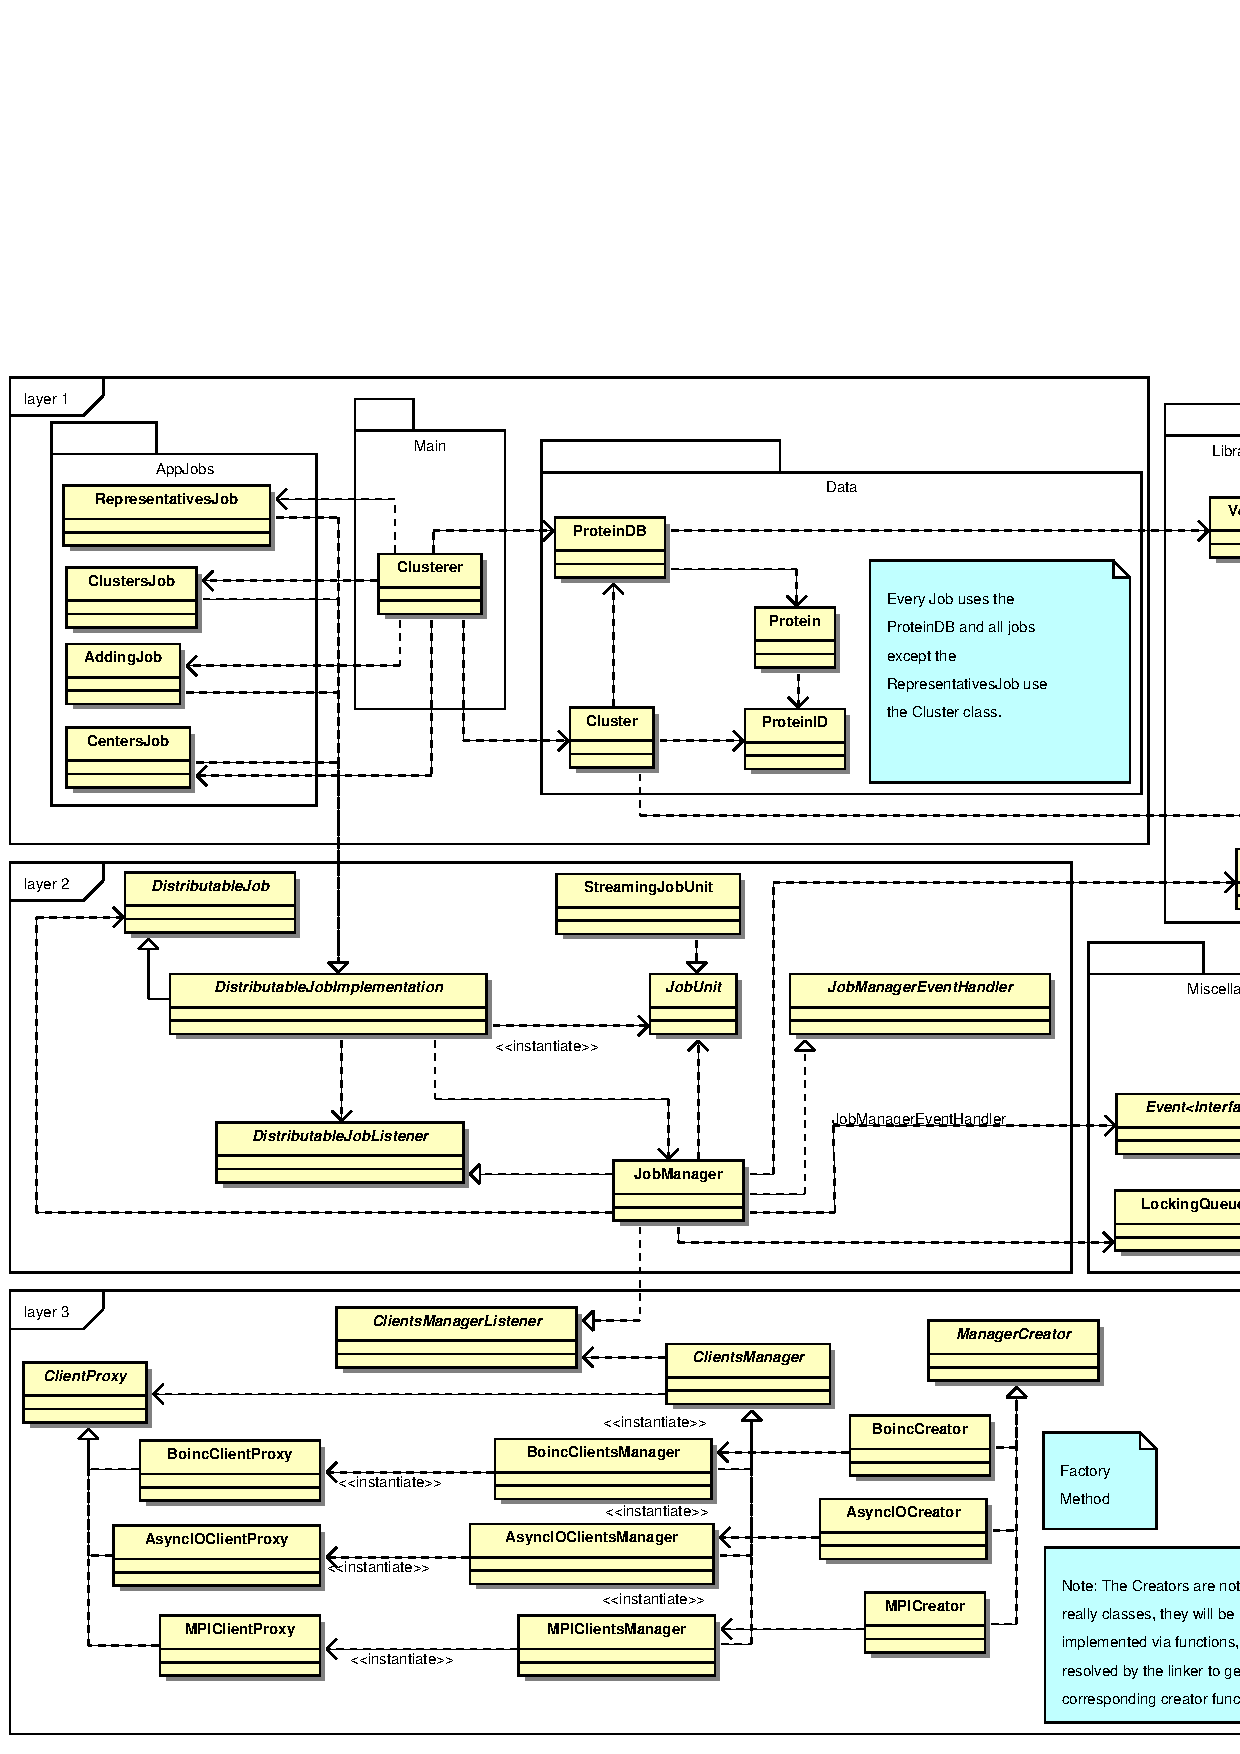
\includegraphics[height=7cm]{images/server-cd.jpg}
    \end{center}
  }

  \frame{
    \frametitle{Diagrama de clases (Cliente)}
    
    \begin{center}
    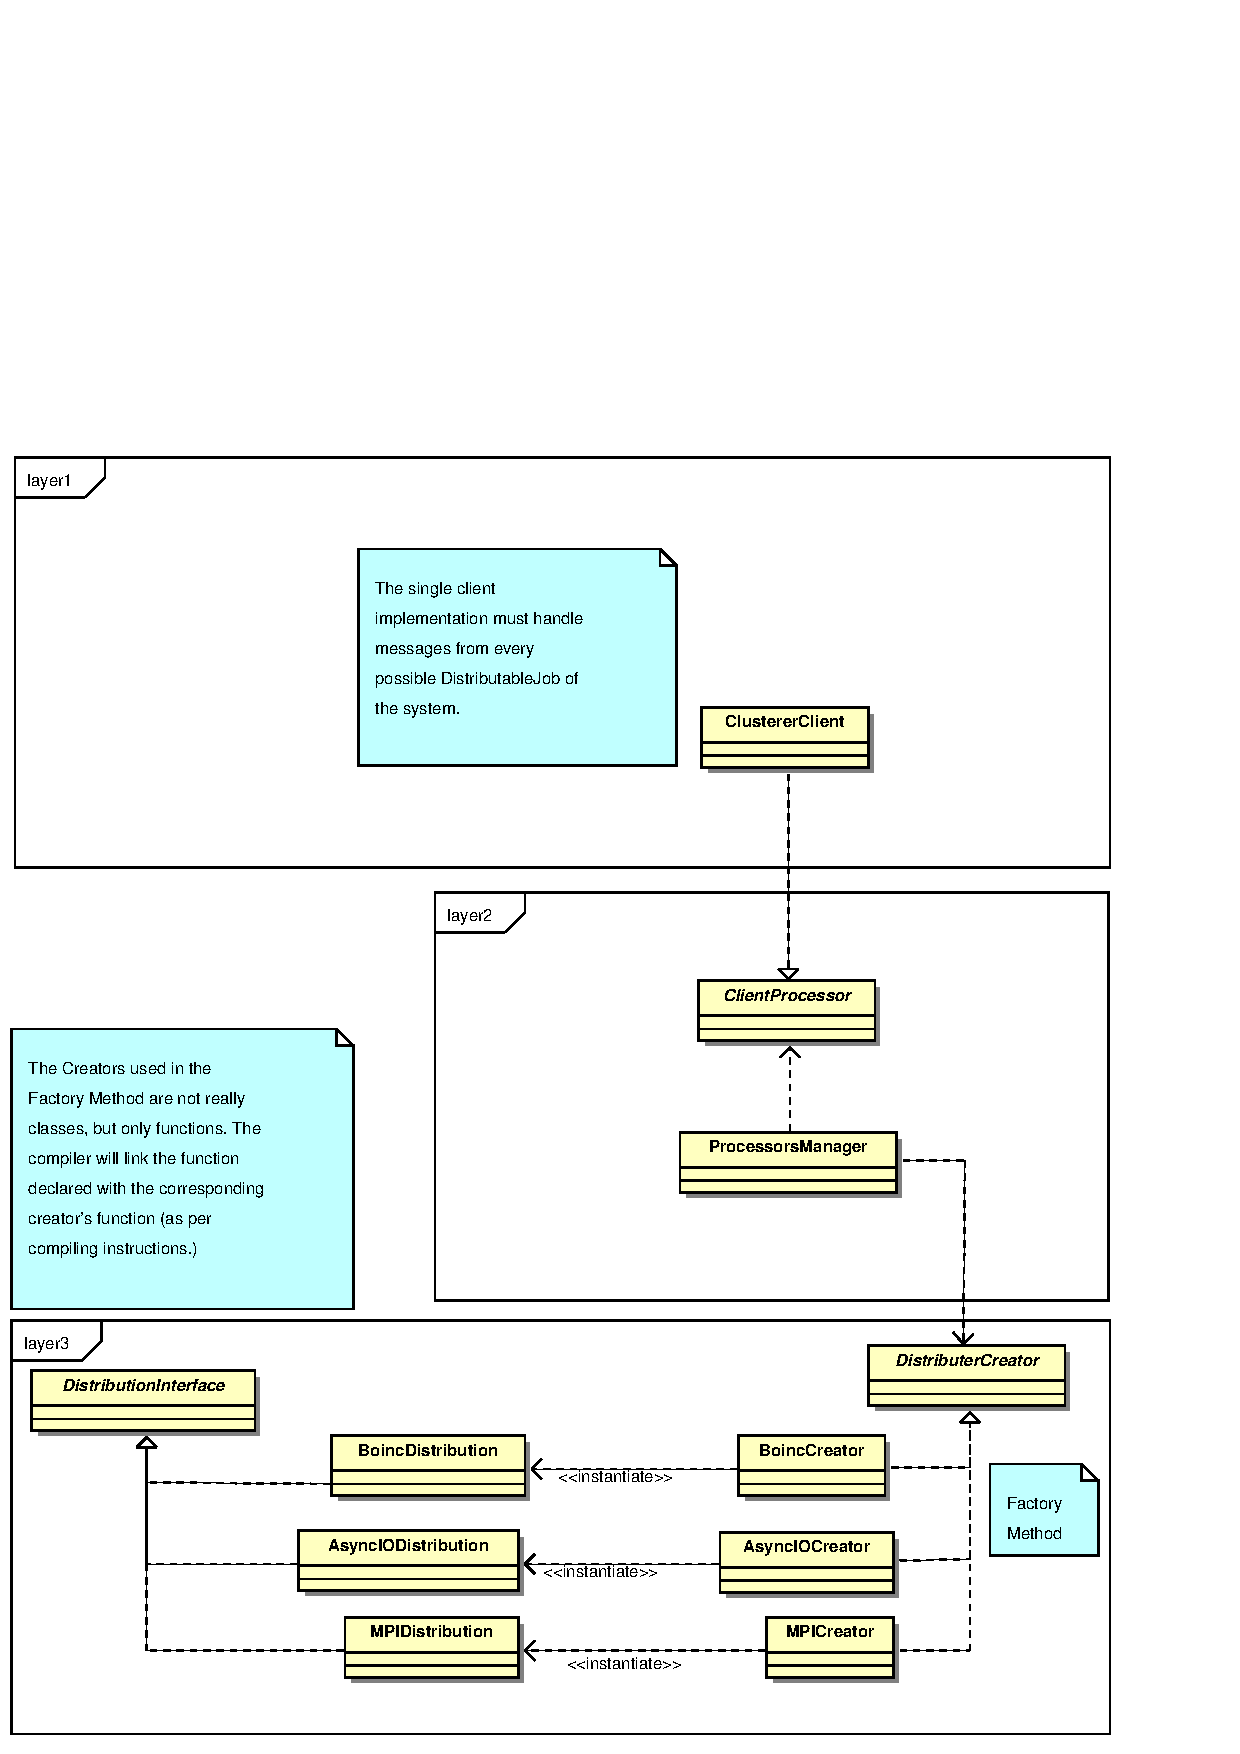
\includegraphics[height=7cm]{images/client-cd.jpg}
    \end{center}
  }

\subsection{Implementaci\'on}

\frame{
  \frametitle{?`C\'omo funciona una aplicaci\'on que usa \textbf{FuD}}
  
  La aplicaci\'on principal que usa a \textbf{FuD} interacciona con el framework de la siguiente manera:
  
  \begin{enumerate}
   \item Crea instancias concretas de trabajos (\texttt{DistributableJob}).
   \pause
   \item Utiliza los m\'etodos provistos por esta interfaz:
     \begin{description}
     \item[run()]: Ejecuta o inicia el trabajo.
     \pause
     \item[wait\_completion()]: Espera (bloqueando) que el trabajo termine.
     \end{description}
  \end{enumerate}
  \pause
  Adem\'as, es la responsabilidad del implementador de la aplicaci\'on:
  \begin{itemize}
   \item Definir el nombre de un trabajo (para logging).
   \pause
   \item Definir el estado de un trabajo.
   \pause
   \item Definir c\'omo se subdivide un trabajo.
   \pause
   \item Definir c\'omo se incorporan resultados de una unidad de trabajo.
  \end{itemize}


}

\begin{frame}[fragile]
\lstset{language=C++}
\begin{lstlisting}[frame=single]
#include "counter.h"
#include "getopt_pp.h"

using namespace fud; using namespace GetOpt;

int main(int argc, char** argv) {
  size_t number(1000); //Default value.
  size_t jobs_n(5);    //Idem.

  GetOpt_pp ops(argc, argv);
  ops >>Option('n', "number", number) >>Option('j',"jobs",jobs_n);

  NumberDatabase* db = new NumberDatabase(number);

  Counter* jobs[jobs_n];
  for (size_t i(0); i < jobs_n; ++i)
      jobs[i] = new Counter(*db,i);

  for (size_t i(0); i < jobs_n; ++i)
      jobs[i]->run();

  jobs[jobs_n-1]->wait_completion();
  std::cout << "Last num: " <<db->current_number() <<std::endl;
}
\end{lstlisting}

\end{frame}


\frame{
  \frametitle{?`C\'omo funciona una aplicaci\'on que usa \textbf{FuD}}
  
  \begin{center}
  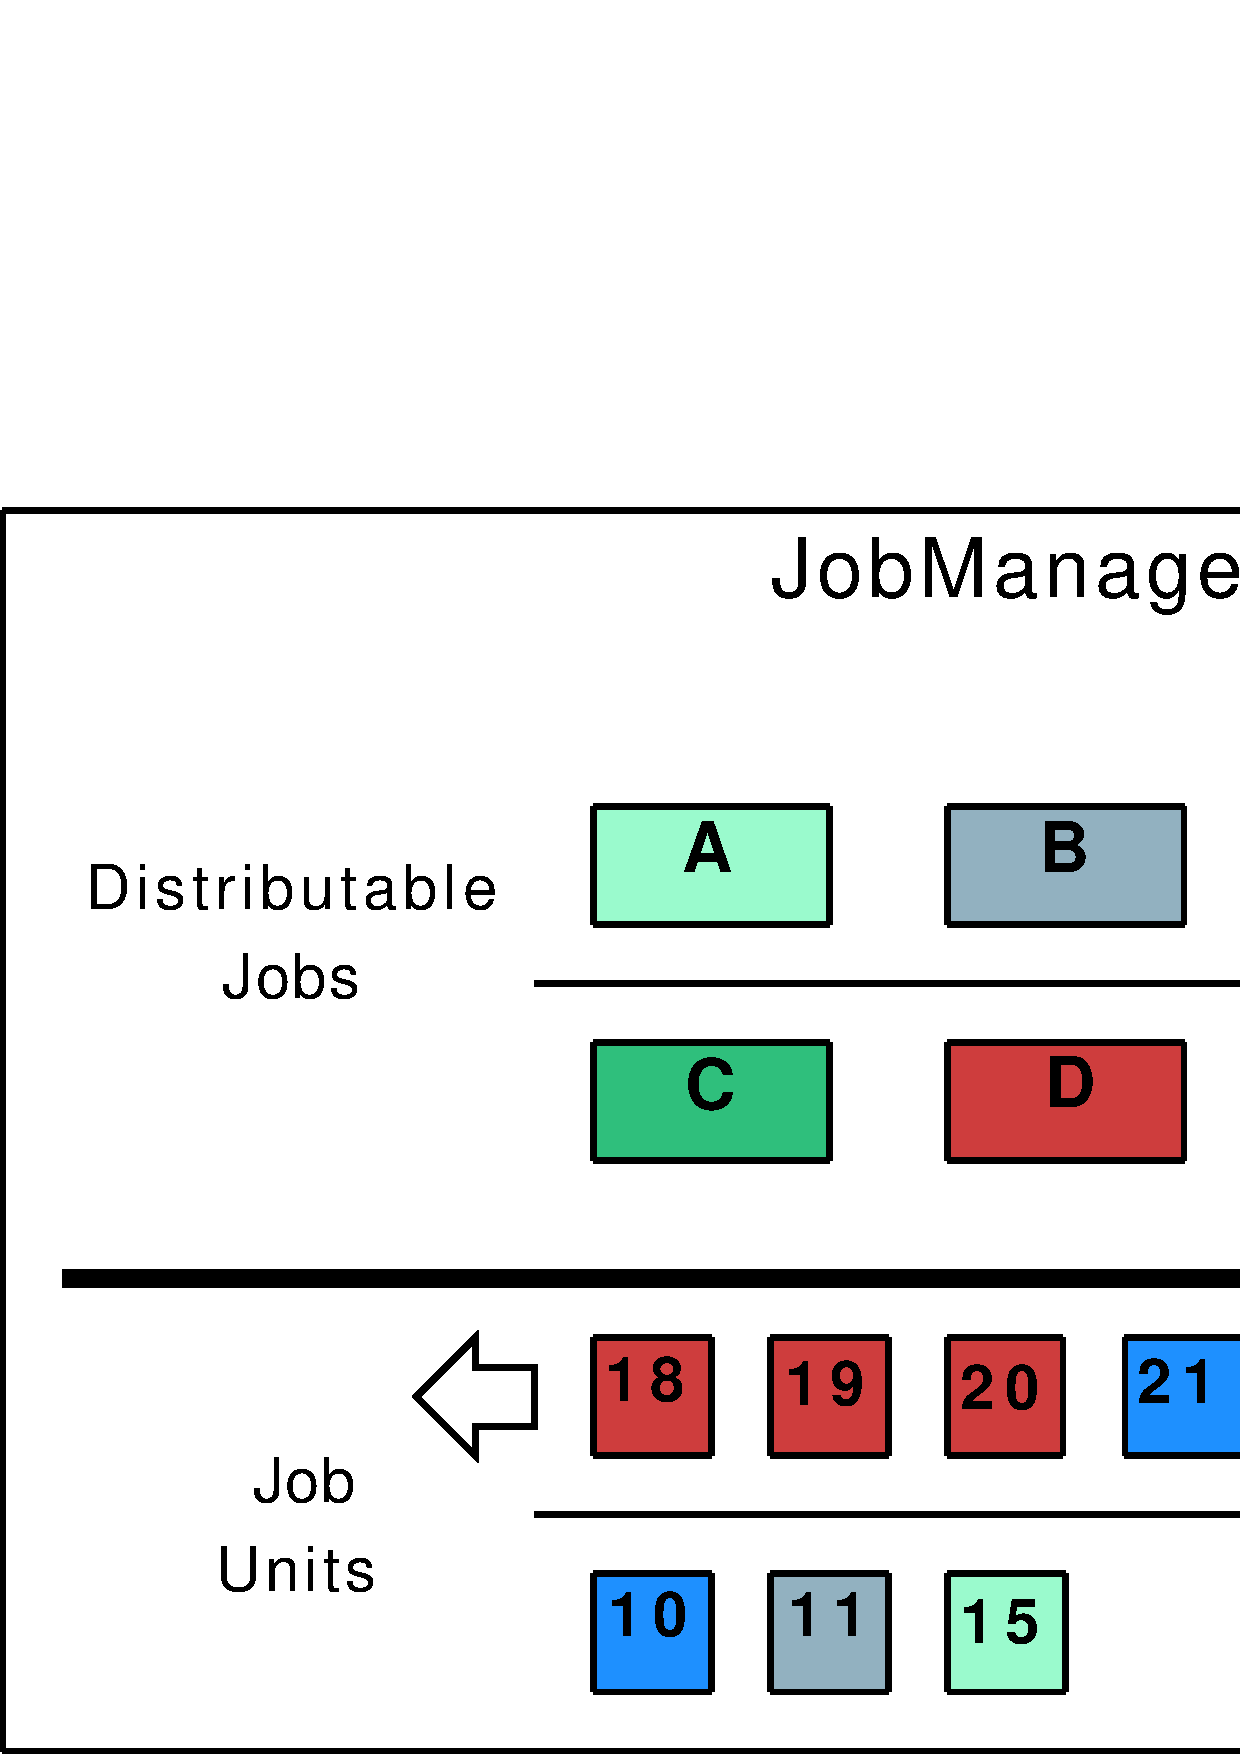
\includegraphics[height=5cm]{images/JobManager.jpg}
  \end{center}

} 

\begin{frame}[fragile]
  \frametitle{Dependecias}
  
  \textbf{FuD} depende de los siguientes paquetes para su compilaci\'on:
  \begin{description}
  \item [Boost]: Una colecci\'on muy completa de librer\'ias para C++.
  \pause
  \item [MiLi]: Colecci\'on sencilla de peque\~nas librer\'ias \'utiles.
  \end{description}
  
  \pause
\lstset{language=C++}
\begin{lstlisting}[frame=single]
/* ... */
template <class T>
bostream& operator<< (T x)
{
    _s.append(reinterpret_cast<char*>(&x), sizeof(T));
    return *this;
}

/* Inserting a string inserts its size first. */
bostream& operator<< (const std::string& s)
{
    (*this) << s.size();
    _s += s;
    return *this;
}
\end{lstlisting}


\end{frame}


  \begin{frame}
  
    \frametitle{M\'etricas}
    
    \begin{center}
      \rowcolors{1}{RoyalBlue!20}{RoyalBlue!5}
      \begin{tabular}{|l|r|r|r|r|c|}
      \hline
      \multicolumn{2}{|c|}{Files} & \multicolumn{3}{|c|}{Line Types} & Percentages \\
      \hline
      \textbf{Type} & \textbf{Count} & \textbf{Blank} & \textbf{Comment} & \textbf{Source} & \small{\textbf{\#Comms./Tot.}}\\
      \hline
      \texttt{C++ source} & 10   &    145  &     360   &    704 & 33.83 \\
      \hline
      \texttt{C++ header} & 16   &    228  &    1223   &    592 &  67.38 \\
      \hline
      \textbf{Total}      &  26  &     373 &     1583  &    1296 & 54.98 \\
      \hline
      \end{tabular}
    \end{center}

  \end{frame}

  \begin{frame}
    \frametitle{Cobertura de c\'odigo}
  \begin{center}
  \rowcolors{1}{RoyalBlue!20}{RoyalBlue!5}
    \begin{tabular}{|l|r|r|c|}
    \hline
    & \multicolumn{2}{|c|}{Lines of Code} & Percentage \\
    \hline
    \textbf{File} & \textbf{Total} & \textbf{Executed} & \textbf{\%} \\
    \hline
    \scriptsize{job\_manager.cpp} & 117 & 95 & 81.2 \\
    \hline 
    \scriptsize{distributable\_job.cpp} & 40 & 39 & 97.5 \\
    \hline 
    \scriptsize{clients\_manager.cpp} & 43 & 38 & 98.37 \\
    \hline 
    \scriptsize{async\_io\_clients\_manager.cpp} & 75 & 56 & 74.67 \\
    \hline 
    \scriptsize{job\_unit.cpp} & 15 & 10 & 66.6 \\
    \hline 
    \textbf{Total} & 290 & 238 & 82.07 \\
    \hline 
    \end{tabular}
  \end{center}
  
  \end{frame}

\section{El Clusterer}

\subsection{Problema}

\begin{frame}
 \frametitle{Definici\'on}

\begin{block}{}
Dados un conjunto de diferentes posibilidades geom\'etricas para una prote\'ina, representadas por un vector de \'atomos, agrupe estos elementos en clusters bajo similitudes geom\'etricas de las posiciones de los \'atomos.
\end{block}

\pause

\begin{block}{}
Dado un conjunto de prote\'inas $D$ y una constante de corte $c$ (en \AA{}). Encuentre una partici\'on $P \subseteq \wp(D)$ de $D$ tal que:
\begin{enumerate}
\item $\forall C \in P$ (cluster) hay un elemento $r \in C$ (representante), tal que todos los miembros de $C$ est\'an a una distanccia menor al corte (usando RMSD) a $r$ y m\'as cercanos a $r$ que a otro representante.
\pause
\item La distancia entre dos representantes es mayor al corte.
\pause
\item La partici\'on es m\'inima.
\end{enumerate}
\end{block}

\end{frame}

\begin{frame}
\frametitle{O($2^n$)}

\begin{alertblock}{}
Pero esto es un problema de minimizaci\'on perteneciente a la clase \textbf{NP-C} (demostraci\'on no presentada).
\end{alertblock}

\pause

Como en nuestro caso, inclusive, el conjunto de datos es potencialmente bastante grande ($n > 10^6$), se debe buscar una aproximaci\'on coherente al problema.

\pause

\begin{block}{}
La versi\'on aqu\'i presentada se caracteriza por ser computacionalmente eficiente, pero todav\'ia mucho trabajo queda por delante para que los resultados de la misma sean de real inter\'es. Esto se cubrir\'a en la secci\'on sobre Trabajo a Futuro.
\end{block}

\pause

Mientras tanto, a continuaci\'on se detalla el algoritmo implementado.

\end{frame}

\begin{frame}[fragile]

\frametitle{Resumen de la implementaci\'on}

Los siguientes pasos resumen el algoritmo:
\begin{exampleblock}{}
 
\begin{enumerate}
\item Encuentra un conjunto de representantes $R$ que cubren $D$.
\pause
\item Crea clusters cuyos representantes sean elementos de $R$.
\pause
\item Calcula la media geom\'etrica de cada cluster.
\pause
\item Asigna nuevos representantes a cada cluster como el m\'as cercano a la media.
\pause
\item Itera entre los pasos 2 (con nuevos representantes) y 4 tantas veces como desee el usuario.
\end{enumerate}

\end{exampleblock}

\pause

Complejidad: O($n^2$) en teor\'ia, pero muy cercano a O($n$) en la pr\'actica (por la naturaleza del conjunto de entrada).

\end{frame}

\subsection{RMSD: disimilitud}

\begin{frame}
\frametitle{RMSD}

La diferencia entre dos prote\'inas se calcula usando RMSD, mediante una media de las sumas de las diferencias entre \'atomos an\'alogos de las estructuras\cite{rmsd}.

\pause
\begin{center}
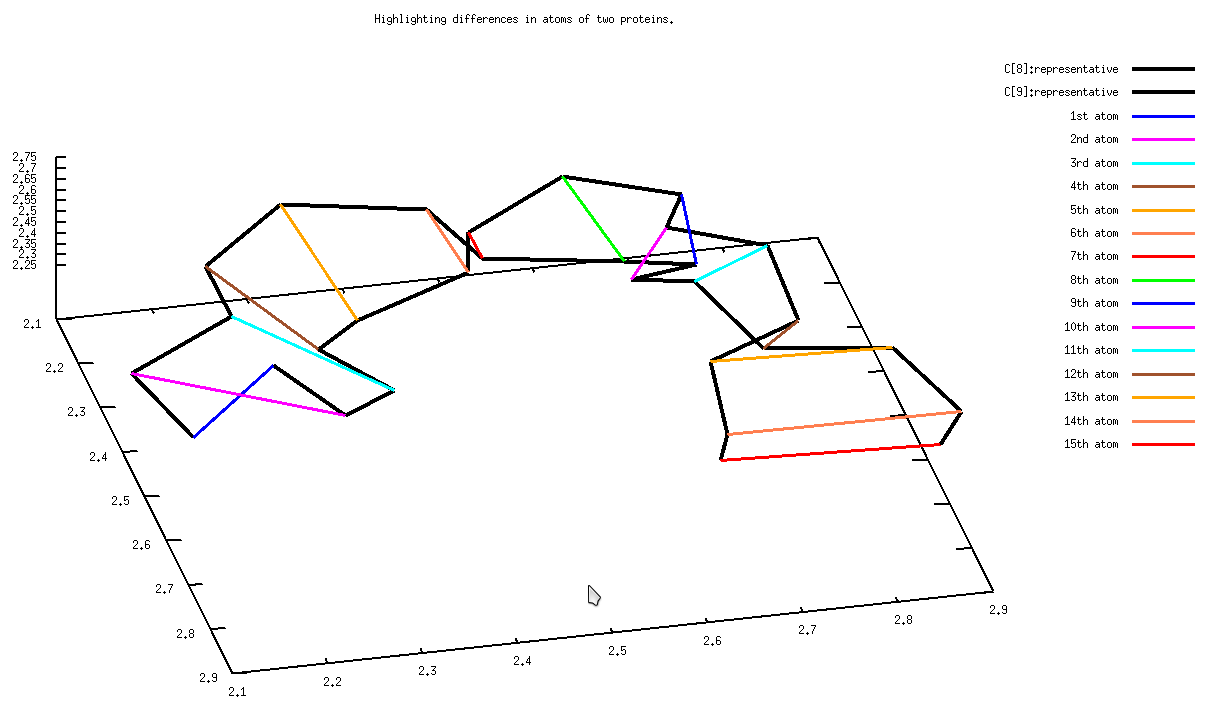
\includegraphics[height=5cm]{images/diff2.png}
\end{center}

\end{frame}

\begin{frame}
 \frametitle{Alternativas}
 
\begin{exampleblock}{RMSD con rotaci\'on}
La comparaci\'on utilizada utiliza superimposici\'on r\'igida de las estructuras. Esto puede ocasionar falsos negativos entre estructuras similares pero rotadas. Es posible rotar de manera que el c\'alculo r\'igido de RMSD es m\'inimo\cite{superimposition}.
\end{exampleblock}

\pause

\begin{exampleblock}{Scaled Gauss Metrics}
Una buena alternativa es utilizar invariantes de nudos para representar la forma de una prote\'ina mediante 30 valores. Este enfoque es bueno para macro-clasificaci\'on\cite{gauss}.
\end{exampleblock}

\pause

Muchos otros enfoques son posibles. En \cite{koehl} se encuentra un buen resumen de t\'ecnicas de comparaci\'on disponibles.

\end{frame}

\subsection{Algoritmo}

\begin{frame}
 \frametitle{Implementando el Clusterer con FuD}
 
 Para implementar el clusterer, en \textbf{FuD} usamos cuatro tipos de trabajos distribu\'ibles:
 \pause
 \begin{block}{}
 \begin{description}
 \item[Representatives]: Iteraci\'on inicial para buscar los representantes.
 \pause
 \item[Clusters]: Arma los clusters con estos representantes.
 \pause
 \item[Adding]: Calcula los centros geom\'etricos de un cluster armado.
 \pause
 \item[Centers]: Selecciona de un cluster el miembro m\'as cercano a la media geom\'etrica para usar como nuevo representante.
 \end{description}

 \end{block}

\end{frame}

\begin{frame}[fragile]
 \frametitle{C\'odigo parcial del main del clusterer}
\lstset{language=C++}
\begin{lstlisting}
ProteinDatabase* db = new ProteinDatabase( input_file.c_str() );

std::vector<Cluster> clusters;

RepresentativesJob* repjob = new RepresentativesJob(*db,cutoff);
repjob->run();
repjob->wait_completion();

ClustersJob* clusters_job = new ClustersJob(*db, repjob->get_marked_ids_vector(), clusters, cutoff);
clusters_job->run();
clusters_job->wait_completion();

AddingJob* adding_job = new AddingJob(*db, clusters, cutoff);
adding_job->run();
adding_job->wait_completion();

CentersJob* centers_job = new CentersJob(*db, clusters, cutoff);
centers_job->run();
centers_job->wait_completion();
\end{lstlisting}

\end{frame}

\subsection*{Salida}

\begin{frame}
 \frametitle{Output del Clusterer}
 
El clusterer permite generar las siguientes salidas:

\begin{description}
 \item [Texto]: Genera un archivo simple de texto con las posiciones de los centros encontrados respecto del archivo original de entrada.
 \pause
 \item [Centros]: Genera un \texttt{.xtc} con todos los centros de los clusters.
 \pause
 \item [Centros geom\'etricos]: Genera un \texttt{.xtc} con la media geom\'etrica de cada cluster.
 \pause
 \item [Clusters]: Genera un \texttt{.xtc} para cada cluster, con el representante como primer elemento.
\end{description}

\pause

Estas salidas pueden luego ser interpretadas por las herramientas, desarrolladas con este prop\'osito, de \texttt{xtc2pdb} y \texttt{xtc2gnuplot}.

\end{frame}


\subsection*{M\'etricas}

\begin{frame}
 \frametitle{M\'etricas I}
 
\begin{center}
\rowcolors{1}{RoyalBlue!20}{RoyalBlue!5}
\begin{tabular}{|l|r|r|r|r|c|}
\hline
\multicolumn{2}{|c|}{Files} & \multicolumn{3}{|c|}{Line Types} & Percentages \\
\hline
\textbf{Type} & \textbf{Count} & \textbf{Blank} & \textbf{Comment} & \textbf{Source} & \small{\textbf{\#Comms./Tot.}}\\ 
\hline
\texttt{C++ source} & 11   &    309  &     469   &    938 & 33.33\\
\hline
\texttt{C++ header} & 10   &    151  &     321   &    441 & 42.12\\
\hline
\textbf{Total}      &  21  &     460 &      790  &    1379 & 36.42\\
\hline
\end{tabular}
\end{center}

\end{frame}

\begin{frame}
 \frametitle{M\'etricas II}
 

\begin{center}
\rowcolors{1}{RoyalBlue!20}{RoyalBlue!5}
\begin{tabular}{|l|r|r|c|}
\hline
 & \multicolumn{2}{|c|}{Lines of Code} & Percentage \\
\hline
\textbf{File} & \textbf{Total} & \textbf{Executed} & \textbf{\%} \\
\hline
\scriptsize{protein\_database.cpp} & 43 & 40 & 93.02 \\
\hline 
\scriptsize{clusterer\_processor.cpp} & 61 & 59 & 96.72 \\
\hline 
\scriptsize{representatives\_job.cpp} & 50 & 49 & 98 \\
\hline 
\scriptsize{clusters\_job.cpp} & 48 & 45 & 93.75 \\
\hline 
\scriptsize{adding\_job.cpp} & 49 & 49 & 100 \\
\hline 
\scriptsize{centers\_job.cpp} & 51 & 51 & 100 \\
\hline 
\textbf{Total} & 302 & 293 & 97.02 \\
\hline
\end{tabular}
\end{center}

\end{frame}

\section{Conclusi\'on y Trabajo a Futuro}

\begin{frame}
 \frametitle{Conclusi\'on}
 
\begin{block}{}
Sobre \textbf{FuD}, postulamos que el dise\~no aqu\'i presentado cumple los requisitos originales. Las aplicaciones de prueba que se han desarrollado para utilizar el framework cubren la mayor\'ia de los tipos de uso posibles.
\end{block}

\pause

\begin{block}{Requisitos}
Desarrollar una aplicaci\'on que use el framework no requiere pensar en t\'erminos de multi-threading o programaci\'on paralela.
\end{block}

\pause
\begin{block}{El clusterer}
Sobre el clusterer, postulamos que la soluci\'on es una aproximaci\'on aceptable. Sin embargo este campo es vasto y un an\'alisis concienzudo del problema de seguro dar\'a a lugares a implementaciones m\'as eficientes y resultados de mayor relevancia. El uso de Scaled Gauss Metrics es una opci\'on prometedora.
\end{block}

\end{frame}

\begin{frame}
\frametitle{Trabajo a Futuro}

Las siguientes tareas deber\'ian llevarse a cabo:
\begin{block}{}
\begin{itemize}
 \item Compilaci\'on con autotools.
 \pause
 \item Uso de BOINC.
 \pause
 \item Uso de MPI para clusters.
 \pause
 \item Clientes multi-threaded.
 \pause
 \item Clientes que se pueden desconectar.
 \pause
 \item Capaz de aplicaci\'on abstractas.
\end{itemize}
\end{block}
\end{frame}


    \begin{frame}[allowframebreaks]{Bibliograf\'ia} 
    \bibliography{biblio}
    \bibliographystyle{apalike}
    \end{frame} 

	\frame {
		\centerline{\Huge{\textbf{?`Preguntas?}}}
	}

	\frame {
		\centerline{\Huge{\textbf{Gracias}}}
	}

    \frame{
      \cite{parallel}
      \cite{svn}
      \cite{tnssitl}
      \cite{texknuth}
      \cite{latex}
      \cite{oosc}
      \cite{clustering}
      \cite{proteins}
      \cite{kmeans}
      \cite{design}
      \cite{pressman}
      \cite{async}
      \cite{faulttolerance}
      \cite{kmeans2}
      \cite{kmeans3}
      \cite{superimposition}
      \cite{gauss}
      \cite{koehl}
      \cite{rmsd}
      \cite{mapreduce}
      \cite{flynn}
      \cite{zait}
      \cite{cplusplus}
      \cite{boinc1}
      \cite{boinc2}
      \cite{proteinsbook}
      \cite{sched1}
      \cite{tanenbaum1}
      \cite{tanenbaum2}
      \cite{sched2}
      \cite{loadbal}
      \cite{macqueen}
      \cite{kmeans-pm}
      \cite{xmeans}
      \cite{murrayetal}
      \cite{proteinclustering}
      \cite{uml}
      \cite{softwarepractices}
      \cite{mpi}
      \cite{openmp}
      \cite{ewd1036}
      \cite{responsibility}
      \cite{boost}
    }

\end{document}

